In this section, I will present a pedagogically interesting 
example which demonstrates several of the programs features. 
The purpose of this chapter is neither to be comprehensive
nor to be particularly detailed. It should instead give a 
sense of the type of analysis that can easily be done with 
this program and motivate the rest of the manual. 
further details and information on any of 
the things of below can be found to the appropriate sections 
of the manual.

David, a user of the program, was studying iron thin films 
using powder diffraction. He was particularly interested in 
measuring the shifts in diffraction peaks of a sample. To 
realize this experimentally, he used a diffraction machine 
to capture the image of the standard calibration crystal 
Lanthanum Hexaboride (LaB6). Without changing the experimental 
parameters, he then imaged many samples for which they wanted 
to measure a shift.

I will describe the steps that would be needed to do this
analysis. First, we will calibrate the diffraction detector.
This is to say that we want to determine the precise 
experimental parameters that characterized the diffraction
machine when the images were captured (for example, the distance
between sample and detector, the energy of the x-rays, etc). Since 
the image of the calibration crystal was taken at the sample
time as the images of interest, the calibration parameters inferred
from the standard crystal can be used in the analysis of the
rest of the crystal.

To perform this calibration, we first opened up the Area 
Diffraction Machine. We are presented with

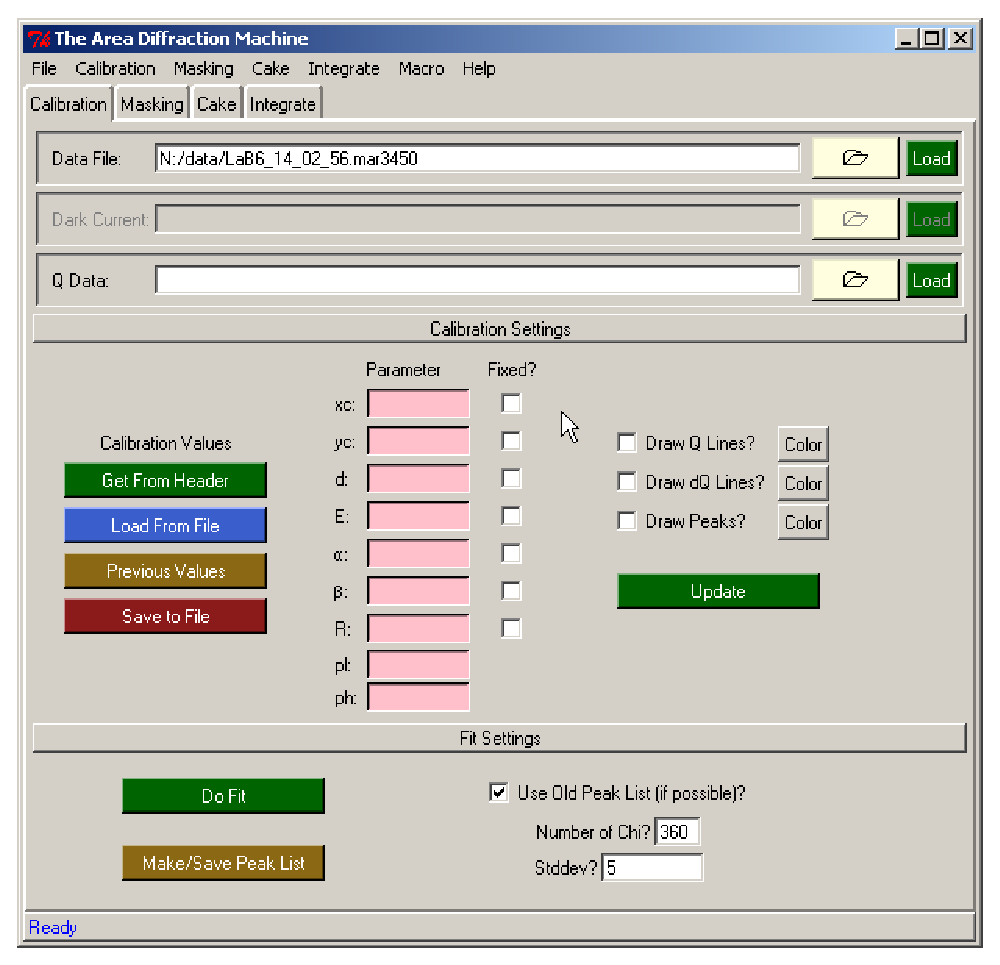
\includegraphics[scale=.75]{figures/calibration_page.eps}

From the \gui{Data File} input, we
load into the program the LaB6 sample file. Once the file
is loaded in, a new window opens up which shows the diffraction
data. This window looks like

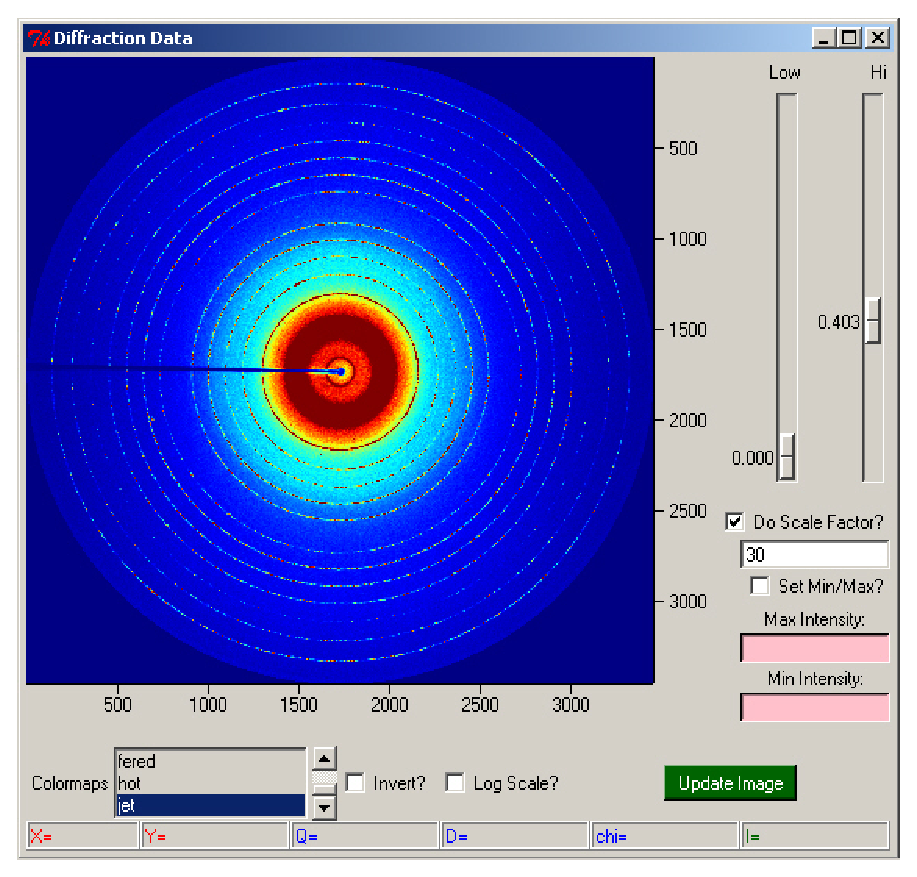
\includegraphics[scale=.75]{figures/diffraction_data_window.eps}

To do the detector calibration, the program must know the 
$Q$ values associated 
with the standard crystal. Since LaB6 is so common, it is
a preset default in the program. We go into the menu bar, 
into the \gui{calibration} menu, into the \gui{Standard Q} menu, 
and then selected Lanthanum Hexaboride. Doing so looks like

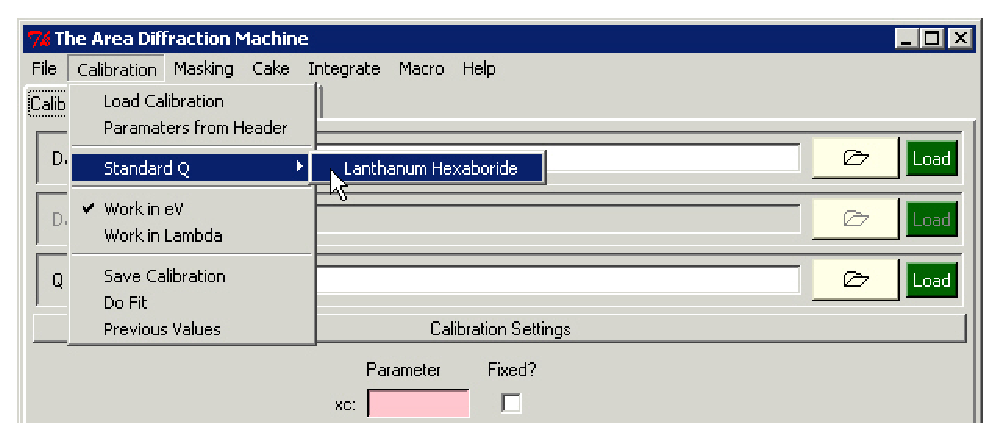
\includegraphics[scale=.75]{figures/standard_q.eps}

(More standard $Q$ files might be added in the future).
In order to perform
image calibration, the program finally needs to know an 
initial guess at the calibration parameters. Although one
could enter these parameters by hand, often times decent
guesses at the experimental parameters are stored in the 
header data inside of the diffraction image. The program
can try to find these header calibration values and put
them into the inputs in the program. To do this, David
pushed the \gui{Get From Header} button. With the image,
the $Q$ values, and an initial guess in the program,
we are ready to do the calibration. 

But first, we want to examine how good the initial guess 
is. To do so, we can select the \gui{Draw Q Lines?}
check box on the Calibration page. When this is selected, 
the program will draw
on top of the diffraction image red lines corresponding
to what diffraction pattern should show up on the
detector (for the given calibration parameters and $Q$
values). For our example, the program displays

%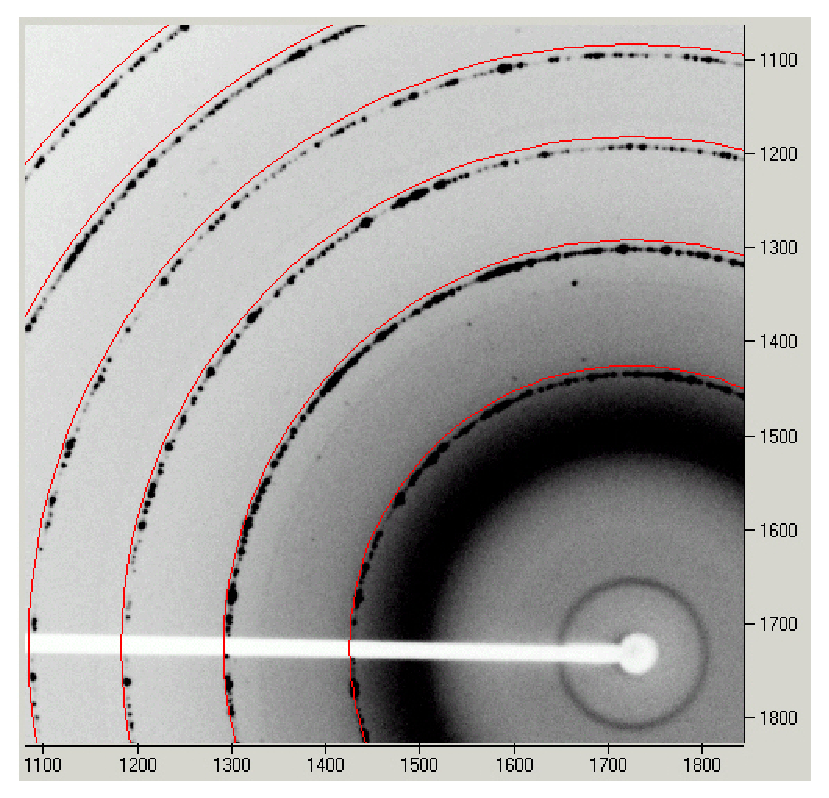
\includegraphics[scale=.75]{figures/bad_calibration_diffraction_image.eps}

Of course, our initial guess isn't
great so the red lines don't match too well with
the loaded patter. The data will look like

We can do an initial cake of the data. A caked plot
is a presentation of the data in a different parameter 
space.  The $x$ axis is $Q$ and the $y$ axis is $\chi$. 
Ideally, if the calibration parameters are known exactly, 
the caked data will show up as many vertical lines. 
We can cake the data by pushing the \gui{AutoCake}
button on the \gui{Cake} page. When we do so, a new cake 
window opens up. For our example, our data looks like

We see that for The caked data with the initial guess 
calibration parameters, our diffraction lines
have a systematic wiggle. It might be hard to see 
with the full image, but by zooming into just one
line, we find the difference to be much more obvious.
This means that our initial guess at 
calibration parameters is not great.

We can now do the calibration. To do so, we push
the \gui{Do Fit} button on the \gui{Calibration}
page. After the calibration finishes, the constant
$Q$ lines drawn on the diffraction image move
so that they are entirely over the diffraction 
pattern. The cake 

This tells us that 


\begin{lstlisting}[caption={'A macro to automate the 
    analysis'}]
Data File:
	C:/Data/
Load From File
    C:/Data/Lab6_cal.dat
Integrate Q Lower?
	0
Integrate Q Upper?
	5
Integrate Number of Q?
	300
Integrate Q-I
Save Integration Data
    PATHNAME/FILENAME_int.dat
\end{lstlisting}

